\documentclass[border=3pt]{standalone}
% Preâmbulo compartilhado pelos diagramas TikZ da aula 8 de IHC (Design de IHC)
\usepackage[T1]{fontenc}
\usepackage[utf8]{inputenc}
\usepackage{lmodern}
\usepackage{amsmath}
\usepackage{xcolor}
\usepackage{tikz}
\usetikzlibrary{arrows.meta,angles,quotes,decorations.pathmorphing,decorations.pathreplacing,calc,
                positioning,shapes.geometric,shapes.misc,backgrounds,fit,
                math}

% Paleta (mesma dos SVGs originais)
% Paleta da disciplina de IHC: acento roxo (#755099), da capa do livro.
% (o nome "dblue" é mantido para não alterar todos os diagramas)
\definecolor{dblue}{HTML}{755099}
\definecolor{dorange}{HTML}{B3541E}
\definecolor{dgreen}{HTML}{4A7C59}
\definecolor{dred}{HTML}{9C4B4B}
\definecolor{dcream}{HTML}{F4F1EA}
\definecolor{dshade}{HTML}{DDD7C9}

% Função gaussiana (não normalizada por padrão de escala visual)
\pgfmathdeclarefunction{gauss}{3}{%
  \pgfmathparse{1/(#3*sqrt(2*pi))*exp(-((#1-#2)^2)/(2*#3^2))}%
}

% Estilos comuns (prefixo d... para não colidir com chaves internas do pgf)
\tikzset{
  >={Stealth[length=2mm]},
  dguide/.style={gray!55, dashed, line width=0.4pt},
  daxis/.style={gray!60, line width=0.7pt, ->},
  dbody/.style={fill=black!3, draw=black!80, line width=1pt},
  dacc/.style={draw=dblue, line width=1pt},
  dlbl/.style={black!55, font=\small},
  dsub/.style={black!45, font=\footnotesize},
  dstate/.style={circle, draw=black!80, fill=dcream, line width=1pt,
                 minimum size=17mm, font=\large, inner sep=1pt},
  dobs/.style={circle, draw=black!80, fill=dshade, line width=1pt,
               minimum size=14mm, font=\large, inner sep=1pt},
  dbox/.style={rounded corners=2pt, draw=black!80, fill=dcream, line width=1pt,
               align=center, inner sep=6pt},
  dop/.style={circle, draw=black!80, fill=white, line width=1pt,
              minimum size=6mm, inner sep=0pt, font=\small},
  dtrans/.style={->, dblue, line width=1pt},
  dmeas/.style={->, dorange, line width=1pt},
  dcurve/.style={line width=1pt, dblue},
  dcurveb/.style={line width=1.4pt, dorange},
}

\begin{document}
\hyphenpenalty=10000 \exhyphenpenalty=10000 \tolerance=9999 \emergencystretch=3em
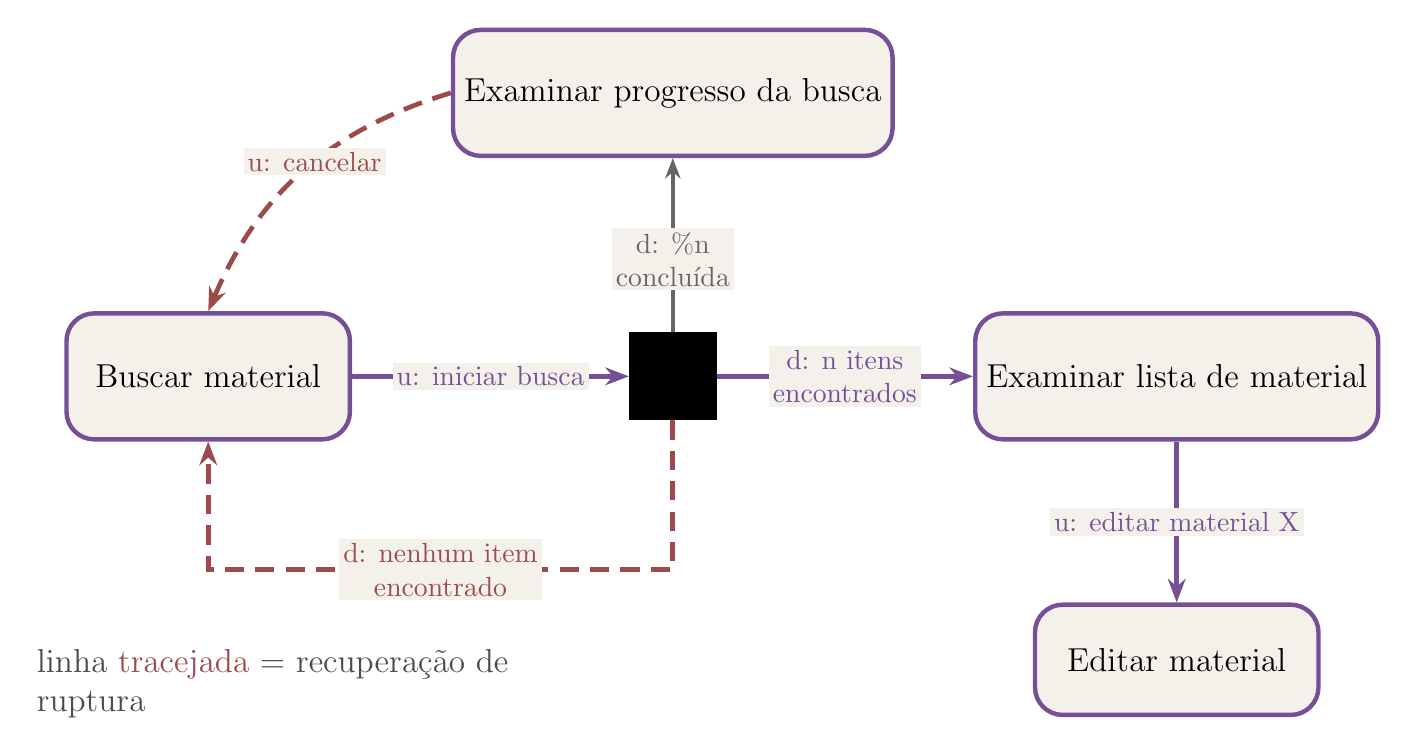
\begin{tikzpicture}[x=1cm,y=1cm]
\tikzset{s/.style={dbox, draw=dblue, rounded corners=10pt, line width=1.6pt, font=\large, inner sep=4pt},
        l/.style={font=\normalsize, fill=dcream, inner sep=1.5pt},
        a/.style={dtrans, line width=1.7pt, -{Stealth[length=3mm]}},
        r/.style={dred, dash pattern=on 7pt off 4pt, line width=1.7pt, -{Stealth[length=3mm]}}}
\node[s, minimum width=3.6cm, minimum height=1.6cm] (b) at (2.4,4.4) {Buscar material};
\node[draw=black, fill=black, minimum size=1.1cm, inner sep=0pt] (x) at (8.3,4.4) {};
\node[s, minimum width=4.2cm, minimum height=1.6cm] (l) at (14.7,4.4) {Examinar lista de material};
\node[s, minimum width=4.4cm, minimum height=1.6cm] (g) at (8.3,8.0) {Examinar progresso da busca};
\node[s, minimum width=3.6cm, minimum height=1.4cm] (e) at (14.7,0.8) {Editar material};
\draw[a] (b.east) -- node[l, pos=0.5] {u: iniciar busca} (x.west);
\draw[a] (x.east) -- node[l, pos=0.5, align=center] {d: n itens\\ encontrados} (l.west);
\draw[black!60, line width=1.5pt, -{Stealth[length=2.6mm]}] (x.north) -- node[l, align=center, pos=0.42] {d: \%n\\ concluída} (g.south);
\draw[r] (g.west) to[bend right=25] node[l, pos=0.45] {u: cancelar} (b.north);
\draw[r] (x.south) -- ++(0,-1.9) -| node[l, pos=0.25, align=center] {d: nenhum item\\ encontrado} (b.south);
\draw[a] (l.south) -- node[l] {u: editar material X} (e.north);
\node[font=\large, black!70, text width=6cm, align=left, anchor=west] at (0.1,0.5) {linha \textcolor{dred}{tracejada} = recuperação de ruptura};
\end{tikzpicture}
\end{document}
